\documentclass[10pt,landscape,a4paper]{article}
\usepackage[utf8]{inputenc}
\usepackage[ngerman]{babel}
\usepackage[T1]{fontenc}
\usepackage{tikz}
\usetikzlibrary{shapes,positioning,arrows,fit,calc,graphs,graphs.standard}
\usepackage[nosf]{kpfonts}
\usepackage[t1]{sourcesanspro}
\usepackage{multicol}
\usepackage{wrapfig}
\usepackage[top=2mm,bottom=2mm,left=2mm,right=2mm]{geometry}
\usepackage[framemethod=tikz]{mdframed}
\usepackage{microtype}
\usepackage{pdfpages}
\usepackage{xfrac}
\usepackage{tikz-cd}
\usepackage{graphicx}
\usepackage{xcolor}
\usepackage{circuitikz}
\tikzset{flipflop DQ/.style={flipflop, scale=1,
         flipflop def={t1=D, t6=Q, c3=1,
         clock wedge size=.3, font=\normalsize}
}}

\graphicspath{ {./img/} }

\let\bar\overline

\begin{document}

\include{inhalt/def}

\small
\begin{multicols*}{3}

\section{Zahlensysteme}
\textbf{Umrechnen von Dezimalzahlen in andere Zahlensysteme}\\\\
Die Dezimalzahl 338 wird ins 5er-System umgewandelt:
\begin{itemize}
    \item 338 : 5 = 67 Rest 3
    \item 67 : 5 = 13 Rest 2
    \item 13 : 5 = 2 Rest 3
    \item 2 : 5 = 0 Rest 2
    \item Rückwärts gelesen: 2323
\end{itemize}
\bigskip
\textbf{Umrechnen von anderen Zahlensystemen in Dezimalzahlen}\\\\
Die Zahl 20022 (3er-System) wird ins Dezimalsystem umgewandelt:
\begin{itemize}
    \item 2 * 3\textsuperscript{0} = 2
    \item 2 * 3\textsuperscript{1} = 6
    \item 0 * 3\textsuperscript{2} = 0
    \item 0 * 3\textsuperscript{3} = 0
    \item 2 * 3\textsuperscript{4} = 162
    \item 2 + 6 + 0 + 0 + 162 = 170
\end{itemize}
\subsection{Negative Zahlen}
\subsubsection{Einerkomplement}
\begin{itemize}
    \item 1. Die Zahl $-6$ wird ins Dualsystem umgewandelt: $6 = 0110$
    \item 2. Das Einerkomplement wird gebildet, indem alle Bits invertiert werden: $1001$
    \item 3. Das Ergebnis ist $-6$ im Einerkomplement: $1001$
    \end{itemize}
\subsubsection{Zweierkomplement}
Wertebereich z.B. 8 Bit: $+127$ bis $-128$, Asymentrie aufgrund der $0$.
\begin{itemize}
    \item 1. Subtraktion ist auch eine Addition mit einer negativen Zahl $2 - 6 = 2 + (-6) = -4$
    \item 2. Die Addition $2 + (-6)$ aufschreiben
    \item 3. Zahlen aus dem Dezimal- ins Dualsystem umschreiben. $2 = 0010 ; 6 = 0110$
    \item 4. Da wir mit einer negativen Zahl rechnen $-6$, müssen wir das Komplement ($1001$) bilden und mit $1$ ($0001$) addieren, damit wir das sogenannte Zweierkomplement erhalten.
    \item 5. Addition vom Komplement und $1$: 
    \begin{align*}
        1001\\
        +0001\\
        \hline
        1010
    \end{align*}
    \item 6. Addition mit der $2$ und $-6$ \\
    $2 + (-6)$:
    \begin{align*}
        0010\\
        1010\\
        \hline
        1100\\
        = -4
    \end{align*}
\end{itemize}
\bigskip
Kurzgesagt: Um ein Zweierkomplement zu bilden muss man invertieren und mit$ 1$ ($0001$) addieren.

Test
\section{Informationstheorie}
\subsection{Typen von Datenquellen}
\subsubsection{Discrete Memoryless Source (DMS)}
\begin{itemize}
    \item Discrete heisst, dass die Quelle (zeitlich) einzelne Ereignisse liefert.
    \item Memoryless bedeutet, die Quelle erinnert sich beim Produzieren
    eines Ereignisses nicht an die Vorgeschichte.
    $\rightarrow$ Die Ereignisse sind (statistisch) unabhängig voneinander
\end{itemize}
\subsubsection{Binary Memoryless Source (BMS)}
\begin{itemize}
    \item Bei dieser Quelle handelt es sich um eine DMS, die aber nur zwei
    verschiedene Ereignisse erzeugt.
    \item Ausgabe ist eine Folge von 0 und 1
\end{itemize}
\subsection{Zweier-Logarithmus}
\begin{equation*}
    x = log_2(K) = \frac{log_{10}(K)}{log_{10}(2)}
\end{equation*}
\subsection{Gleiche Wahrscheinlichkeit}
\begin{itemize}
    \item Je mehr Fälle es gibt, desto seltener tritt ein bestimmtes Ereignis ein.
    \item Je seltener ein Ereignis ist, desto höher ist sein Informationsgehalt.
    \item $N$ sei wieder die Anzahl der möglichen Ereignisse. Wenn alle Ereigniswerte $x_n$ die Gleiche
    Auftretungswahrscheinlichkeit $P(x_n)$ haben, gilt:
    \begin{equation*}
        P(x_n) = \frac{1}{N} \rightarrow N = \frac{1}{P(x_n)}
    \end{equation*}
\end{itemize}
\subsection{Informationsgehalt von Ereignissen}
\begin{itemize}
    \item Je seltener ein Ereignis eintritt, desto grösser ist der
    Informationsgehalt (Überraschungseffekt)
    \item Die folgende Formel gilt allgemein:
    \begin{equation*}
        I(x_n) = log_2(\frac{1}{P(x_n)})
    \end{equation*}
\end{itemize}
\subsection{Entropie}
Den mittleren Informationsgehalt von Quellen nennt man Entropie:
\begin{equation*}
    H(X) = \sum_{n=0}^{N-1} P(x_n) \cdot I(x_n) = \sum_{n=0}^{N-1} P(x_n) \cdot log_2(P(x_n))
\end{equation*}
Die Masseinheit der Entropie ist $Bit/Symbol$.
\subsubsection{Entropie Binary Memoryless Source}
Eine BMS kennt nur zwei Symbole. Ist $p$ die Auftretungswahrscheinlichkeit des eines Symbols, folgt dass $(1-p)$ jene des anderen Symbols ist.
\begin{equation*}
    H_b = p  \cdot log_2(\frac{1}{p}) + (1-p)  \cdot log_2(\frac{1}{1-p})
\end{equation*}
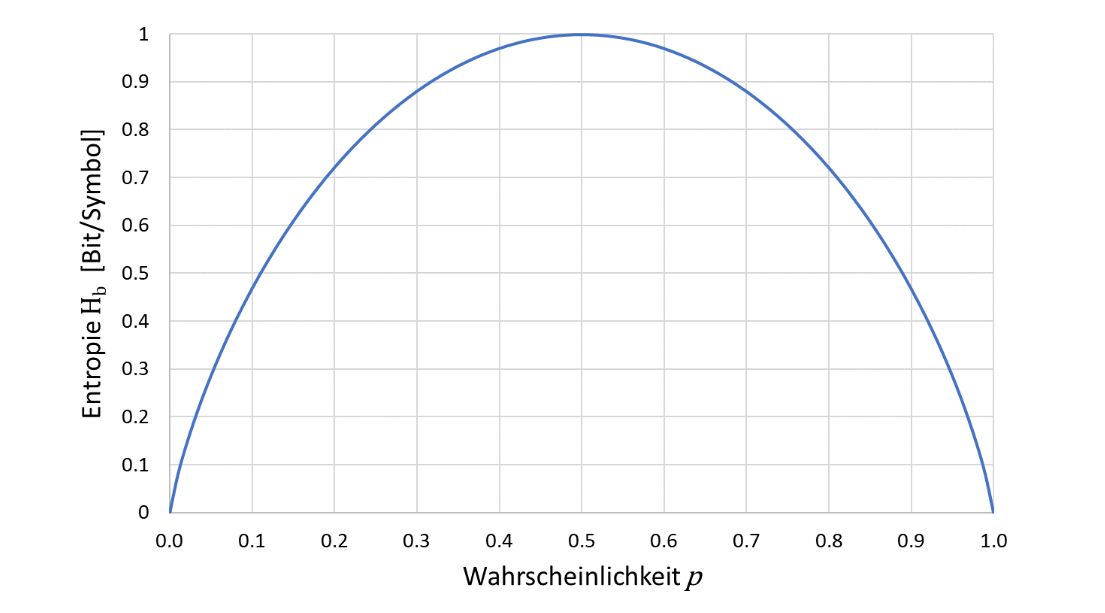
\includegraphics[scale=0.25]{binaere_Entropiefunktion}

\section{Quellencodierung}
\subsection{Redundanz}
\subsubsection{Codewortlänge $\ell_n$}
\begin{center}
	\begin{tabular}{ c c c }
		Symbol & Code           & Codewortlänge    \\
		$x_0$  & $c_0 = (10)$   & $\ell_0 = 2 Bit$ \\
		$x_1$  & $c_1 = (110)$  & $\ell_1 = 3 Bit$ \\
		$x_2$  & $c_2 = (1110)$ & $\ell_2 = 4 Bit$
	\end{tabular}
\end{center}
\subsubsection{Mittlere Länge der Codierung $L$}
\begin{equation*}
	L = \sum_{n=0}^{N-1} P(x_n) \cdot \ell_n
\end{equation*}
\subsubsection{Redundanz $R$}
In $Bit/Symbol$:
\begin{equation*}
	R = L - H(X)
\end{equation*}
\subsubsection{Theorem zu Quellencodierung}
\begin{itemize}
	\item Falls $R > 0$, dann kann verlustfrei komprimiert werden.
	\item Falls $R \leq 0$, dann kann nur verlustbehaftet komprimiert werden.
\end{itemize}
\subsection{Kompressionsrate}
\begin{align*}
	R = \frac{\text{Grösse komprimierte Daten}}{\text{Grösse Originaldaten}} \\
	\text{Kompressionsrate } R \neq \text{Redundanz } R
\end{align*}
\subsection{Lauflängencodierung}
Lauflängencodierung oder Run-Length Encoding (RLE) ist eine einfache Methode
zur verlustfreien Datenkompression.
\begin{itemize}
	\item Marker bestimmen, z.B. selten genutzes Zeichen.
	\item Marker und Anzahl der Wiederholungen speichern.
\end{itemize}
\begin{verbatim}
    Hier verwenden wir als Marker z.B. Z:
    Orginal: ASKEEEEEEEEEEFEIIIIIPPPP ...
    Codiert: ASKZ10EZ05IZ04P ...
\end{verbatim}
\subsection{Huffman-Codierung}
Um Huffman-Codierung anzuwenden, muss die Wahrscheinlichkeit $P(x_n)$ der Symbole bekannt sein.
\begin{itemize}
	\item Ordne alle Symbole nach aufsteigenden Auftretenswahrscheinlichkeiten auf einer Zeile. Dies sind die Blätter des Huffman-Baums.
	\item Notiere unter jedes Blatt seine Wahrscheinlichkeit.
	\item Schliesse die beiden Blätter mit der kleinsten Wahrscheinlichkeit an einer gemeinsamen Astgabel an und ordne dem Ast die Summe der Wahrscheinlichkeiten der beiden Blätter zu.
	\item Wiederhole den vorherigen Schritt mit Blättern und Ästen so lange, bis nur noch der Stamm des Baums übrig bleibt.
	\item Nun wird bei jeder Astgabel dem einen Zweig eine 0 und dem anderen eine 1 zugeordnet. (Die Zuordnung ist frei wählbar, muss aber über den ganzen Baum einheitlich sein).
	\item Nun werden auf dem Pfad vom Stamm zu jedem Blatt die Nullen und Einsen ausgelesen und von links nach rechts nebeneinander geschrieben. Dies sind die Huffman-Codeworte.
\end{itemize}
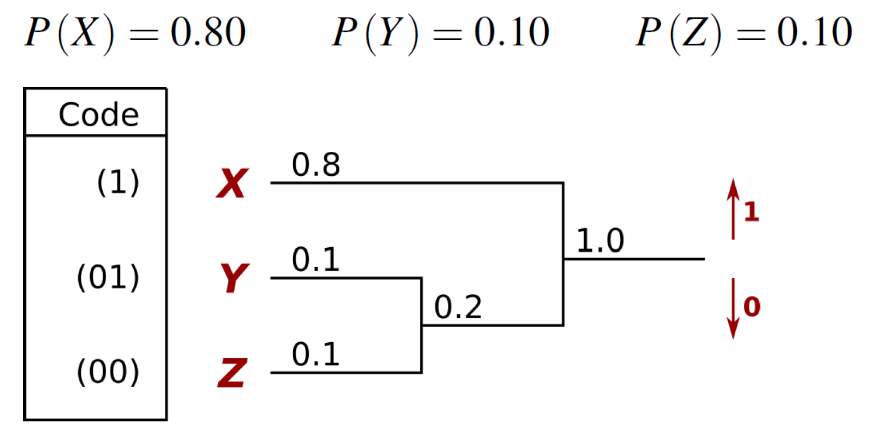
\includegraphics[scale= 0.4]{huffman}
\subsection{LZ77}
Für LZ77 ein Suchbuffer $n_{s}$ und Vorschaubuffer $n_{v}$ definiert.
Der Token hat das Format (Offset, Länge, Zeichen).
\begin{itemize}
    \item Alle Zeichen werden durch Tokens fixer Länge ersetzt.
    \item Zur Bildung der Tokens werden die Daten durch ein Sliding Window, bestehend aus Such- und Vorschaubuffer, geleitet.
    \item Im Such-Buffer wird die längste Übereinstimmung mit dem Vorschau-Buffer als Token ausgegeben.
    \item Keine Übereinstimmung: Token $(0, 0, \text{Zeichen})$ wird verwendet.
\end{itemize}
\begin{center}
	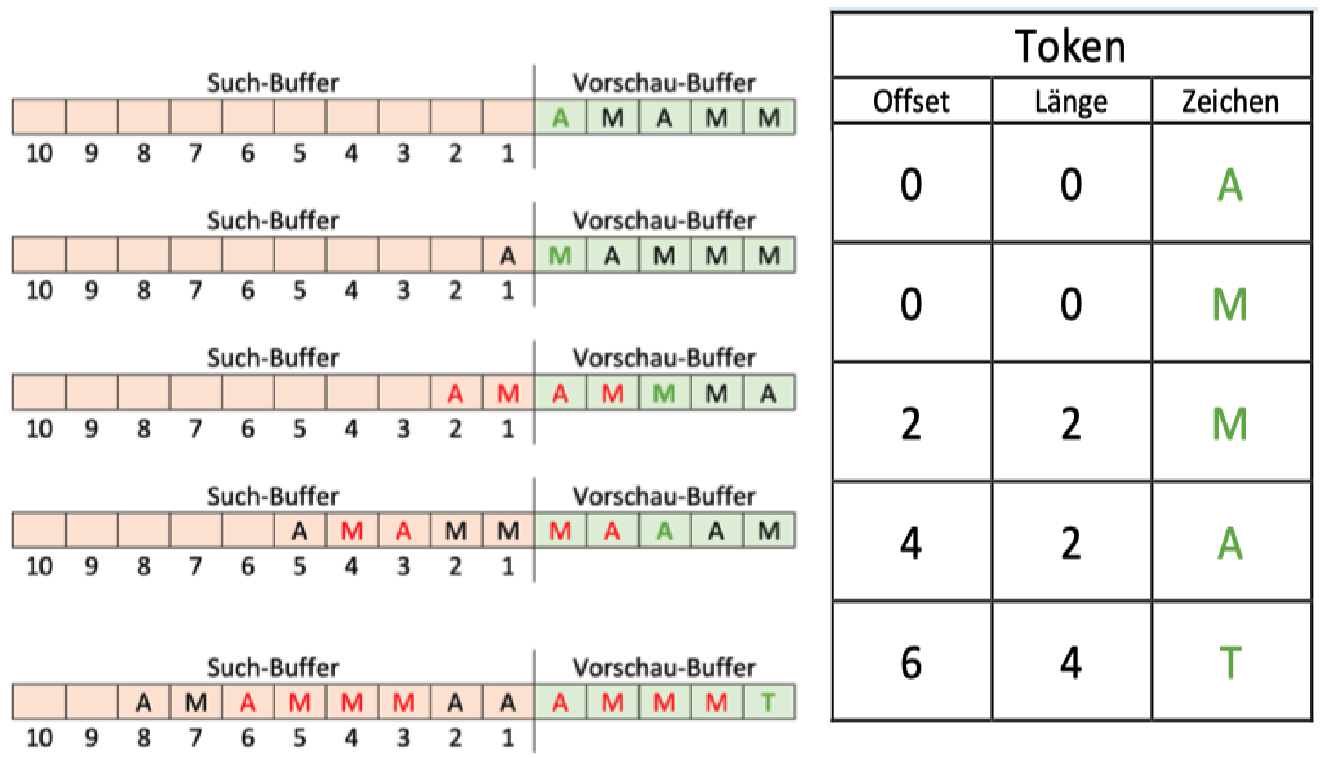
\includegraphics[scale=0.27]{lz77}
\end{center}

\subsubsection{Einzelne Tokengrösse}
\begin{align*}
\text{Grösse Such-Buffer} + \text{Grösse Vorschau-Buffer} + \text{Zusätzliches Zeichen}
\end{align*}

\subsubsection{Gesamt}
\begin{align*}
\text{Anzahl Tokens} \times \text{Tokengrösse}
\end{align*}

\subsubsection{Kompressionsrate}
\begin{align*}
R = \frac{\text{LZ77 Codierung in Bits}}{\text{String ohne Codierung in Bits}}
\end{align*}

\noindent
\textbf{Beim Token:} Die Buffergrösse ist jeweils $\text{roundUp}(\log_2(N))$, wobei $N$ die Zahl ist, bis zu der wir maximal zählen können. \\
Beispiel Such-Buffer (1 bis 10): $\text{roundUp}(\log_2(10)) = 3.321\ldots = 4$ Bit
\subsubsection{Decoding}
\begin{itemize}
	\item Start mit leerem Such-Buffer
	\item Bei Tokens ohne Referenz in den Such-Buffer einfach Zeichen ausgeben und in Such-Buffer schieben
	\item Bei Tokens mit Referenz in den Such-Buffer wird zunächst der referenzierte String ausgegeben und das Symbol im Token
\end{itemize}

\subsection{LZW}
\subsubsection{Verfahren}
\begin{itemize}
	\item Basic vorinitialisiertes Wörterbuch (Bsp: Einzelsymbole von ASCII), Einzelne Zeichen sind immer im Wörterbuch vorhanden!
	\item String von links nach rechts lesen, bis der gelesene Teilstring nicht mehr im Wörterbuch vorkommt
	\item Token enthält nur den Index des schon bestehenden Eintrags im Wörterbuch, nicht aber das neue Zeichen
\end{itemize}
\begin{center}
	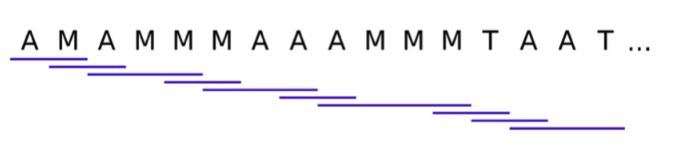
\includegraphics[scale=0.5]{lzw1}
\end{center}
\subsubsection{Decoding}
\begin{center}
	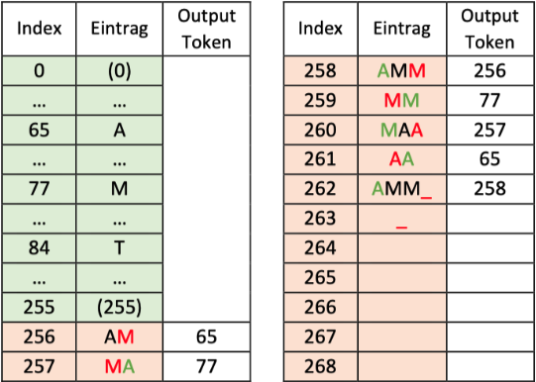
\includegraphics[scale=0.6]{lzw2}
\end{center}
Das Zeichen ganz rechts vom Eintrag wird erst bei dem
nächsten Token übertragen (Überlappung)
\section{Kanalcodierung}
\subsection{Bitfehlerwahrscheinlichkeit $\varepsilon$}
$\varepsilon$ ist die Wahrscheinlichkeit, dass ein Bitfehler auftritt (BER - Bit Error Rate).
\begin{itemize}
	\item Alle Bits falsch: $BER = 1$
	\item Kein Bit falsch: $BER = 0$
	\item 1 von 2 Bits falsch: $BER = 0.5$
	\item 1 von 1000 Bits falsch: $BER = 0.001$
\end{itemize}
\subsection{Binary Symmetric Channel (BSC)}
Bei $x_1$ und $x_0$ kommen jeweils 0 oder 1 hinen. Die Wahrscheinlichkeit, dass ein Bitfehler auftritt, ist $\varepsilon$.
Die Wahrscheinlichkeit dass kein Bitfehler auftritt, ist $1 - \varepsilon$.
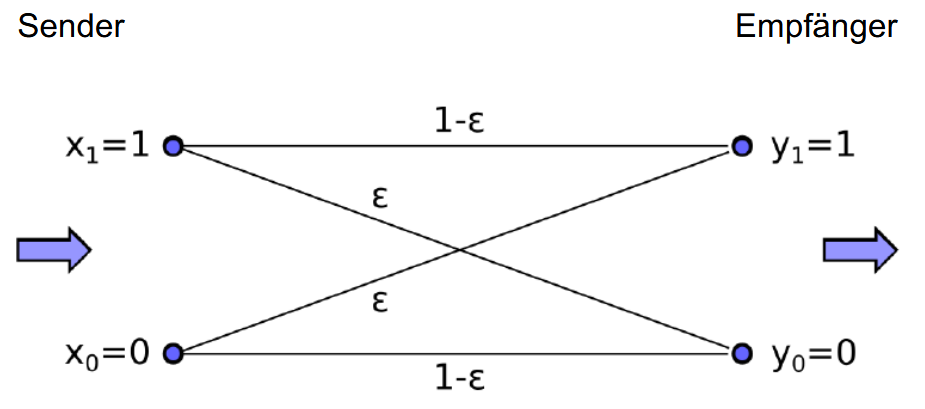
\includegraphics[scale=0.4]{bsc}
\subsubsection{Erfolgswahrscheinlichkeit}
\begin{align*}
	P_{0,N} = \frac{A_N}{A} = (1 - \varepsilon)^N
\end{align*}
\subsubsection{Fehlerwahrscheinlichkeit}
Auf $N$ Datenbits:
\begin{align*}
	1 - P_{0,N} = 1 - (1 - \varepsilon)^N
\end{align*}
Wobei für $N \cdot \varepsilon \ll 1$ folgende Näherung gilt: $1 - (1 - \varepsilon)^N \approx ( 1 - N \cdot \varepsilon)$
\subsubsection{Mehr-Bit-Fehlerwahrscheinlichkeit}
\begin{itemize}
	\item $\binom{N}{F}$: Anzahl der Möglichkeiten, $F$ Fehler in $N$ Bits zu platzieren.
	\item $\varepsilon^F$: Wahrscheinlichkeit, dass $F$ Fehler auftreten.
	\item $(1 - \varepsilon)^{N-F}$: Wahrscheinlichkeit, dass Alle restlichen Bits $N-F$keinen Fehler haben.
\end{itemize}
\begin{align*}
	P_{F,N} = \binom{N}{F} \cdot \varepsilon^F \cdot (1 - \varepsilon)^{N-F}
\end{align*}
$\binom{N}{F} = \frac{N!}{F! \cdot (N-K)!}$ bzw. $\binom{6}{2}$ rechnet man wie folgt:
\begin{align*}
	\binom{6}{2} = \frac{6!}{2! \cdot (6-2)!} = \frac{6 \cdot 5 \cdot 4 \cdot 3 \cdot 2 \cdot 1}{2 \cdot 1 \cdot (4 \cdot 3 \cdot 2 \cdot 1)}
	= \frac{6 \cdot 5 \cdot \cancel{4 \cdot 3 \cdot 2 \cdot 1}}{2 \cdot 1 \cdot \cancel{(4 \cdot 3 \cdot 2 \cdot 1)}}  = \frac{6 \cdot 5}{2 \cdot 1} = 15
\end{align*}
\subsubsection{Coderate $R$}
\begin{itemize}
	\item Die Coderate $R$ ist das Verhältnis von Nutzdatenbits zu gesendeten Bits.
	\item $K$ ist die Anzahl der Nutzdatenbits und $N$ die Anzahl der gesendeten Bits.
	\item Z.B. $Paritaetsbits + Informationsbits = N$\\ und $K = Informationsbits$.
\end{itemize}
\begin{align*}
	R = \frac{K}{N}
\end{align*}
\subsubsection{Kanalkapazität $C$}
Die Kanalkapazität $C$ in $bit/bit$ ist die maximale Datenrate, die über einen Kanal übertragen werden kann.
\begin{align*}
	C_{BSC}(\varepsilon) = 1 - H_b(\varepsilon)
\end{align*}
\subsubsection{Kanalkodierungstheorem}
Möchte man die Restfehlerwahrscheinlichkeit eines Fehlerschutzcodes beliebig klein machen,
so muss $R < C$ sein.
\subsection{Hamming-Distanz}
Die Hamming-Distanz $d_H$ ist die Anzahl der unterschiedlichen Bits zwischen zwei Codewörtern.\\
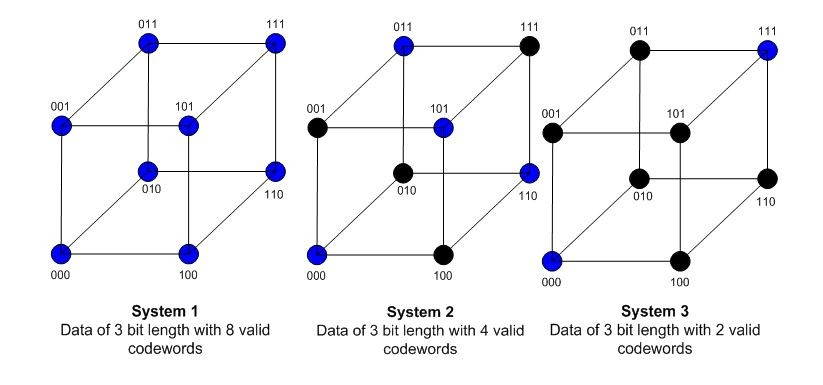
\includegraphics[scale=0.45]{hamming}
\subsubsection{Eigenschaften}
\begin{itemize}
	\item \textbf{Systematisch}: Ein Code ist Systematisch wenn die Nutzdatenbits unverändert im Codewort übernommen werden.
	      Hierfür müssen legendlich z.B. die Paritätsbits entfernt werden.
	\item \textbf{Linear}: Ein Code ist linear wenn jede Kombination ($EXOR$) von Codewörtern wieder ein Codewort ist.
	\item \textbf{Zyklisch}: Ein zyklischer Code ist eine spezielle Art eines linearen Codes, bei dem jede
	      zyklische Verschiebung eines Codeworts ebenfalls ein gültiges Codewort ist.
	\item \textbf{Perfekt}: Ein Code heisst ein «perfekter Code», wenn jedes empfangene Wort $w$
	      genau ein Codewort $c$ hat, zu dem es eine geringste Hamming-Distanz
	      hat und zu dem es eindeutig zugeordnet werden kann.
\end{itemize}
\subsection{Paritätscheck}
\subsubsection{1D Paritätscheck}
Ein Parity-Bit bestimmt, ob die Anzahl Einer in einem Codewort gerade oder ungerade ist.
Even und Odd Parity sind gleichwertig, wobei nur even parity lineare Codes ermöglicht.
\subsubsection{2D Paritätscheck}
Ein 2D Paritätscheck...
\begin{itemize}
	\item ...ist ein Paritätscheck, der auf zwei Dimensionen angewendet wird.
	\item ...kann einen Fehler in einer Zeile oder Spalte erkennen und korrigieren.
	\item ...kann zwei Fehler erkennen, aber nicht korrigieren.
	\item ...kann drei Fehler nicht erkennen.
\end{itemize}
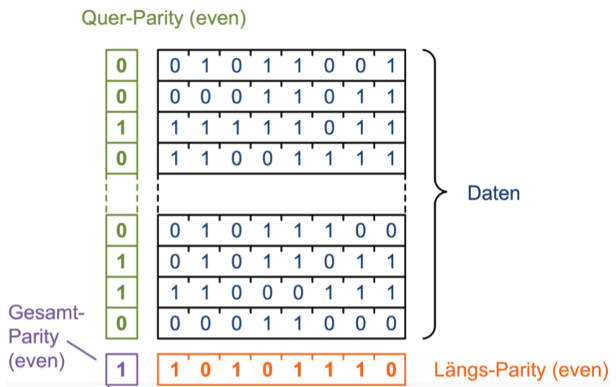
\includegraphics[scale=0.5]{2d_parity}

\subsection{CRC}
\subsubsection{CRC-Polynomdivision}
\begin{itemize}
	\item Nutzdatenwort: $111010100$
	\item Generatorpolynom: $x^3 + x^2 + 1 \Rightarrow$ $\textcolor{blue}{1101}$
	\item Nutzdatenwort mit Nullen (Grad des Generatorpolynoms [3]) erweitern: $111010100\textcolor{red}{000}$
	\item Rest bestimmen durch Division: $100$
	\item Rest an Nutzdatenwort anhängen: $111010100\textcolor{red}{100}$
\end{itemize}
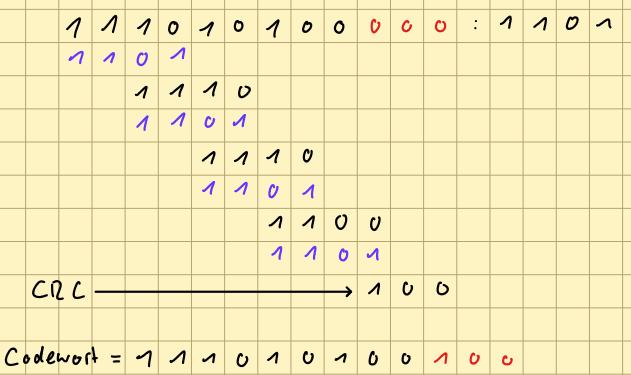
\includegraphics[scale=0.55]{crc_div}
\subsection{Blockcodes}
Lineare Blockcodes werden über eine Generatormatrix
definiert. Das Codewort entsteht indem die Daten mit der
Generatormatrix multipliziert werden:\\
\begin{align*}
    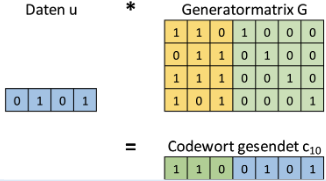
\includegraphics[scale=1]{blockcode1}
\end{align*}
\subsubsection{Bildung Generatormatrix}
\begin{align*}
    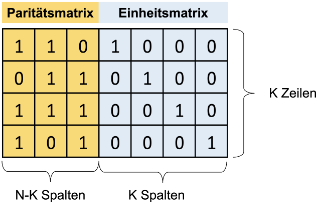
\includegraphics[scale=0.8]{blockcode2}
\end{align*}
Die Paritaetsbits (Zeilen) müssen voneinander linear unabhängig sein.
Für Hamming-Codes gilt: Jede Zeile hat gleich viele Einsen wie $d_{min}$.
\begin{align*}
    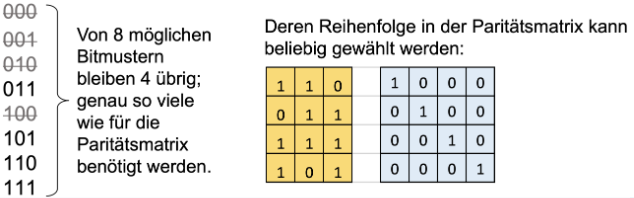
\includegraphics[scale=0.6]{blockcode3}
\end{align*}
\subsubsection{Bildung Prüfmatrix}
\begin{align*}
    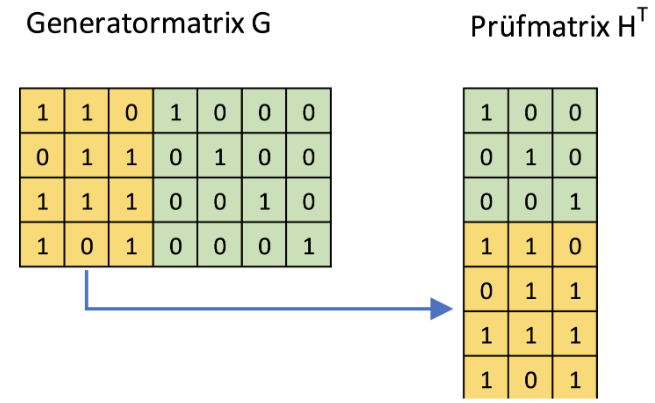
\includegraphics[scale=0.5]{blockcode4}
\end{align*}
\begin{align*}
    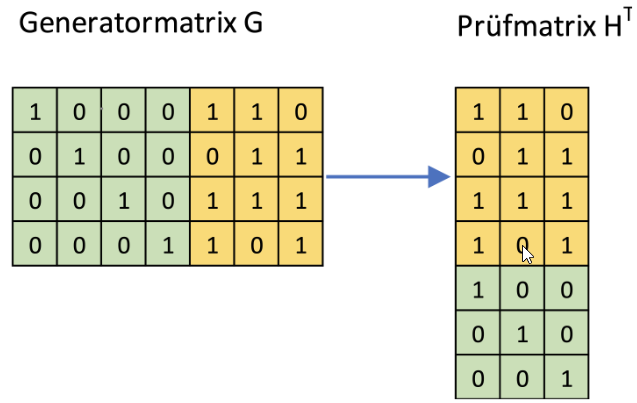
\includegraphics[scale=0.5]{blockcode5}
\end{align*}

\subsection{Faltungscodes}
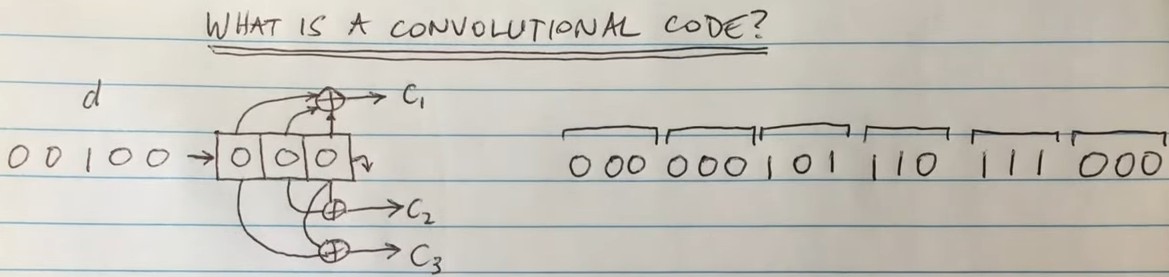
\includegraphics[scale=0.31]{faltungscode}
\subsubsection{Trellis Diagramm}
\vspace*{20\baselineskip}
\section{Faltungscodes}
\begin{center}
    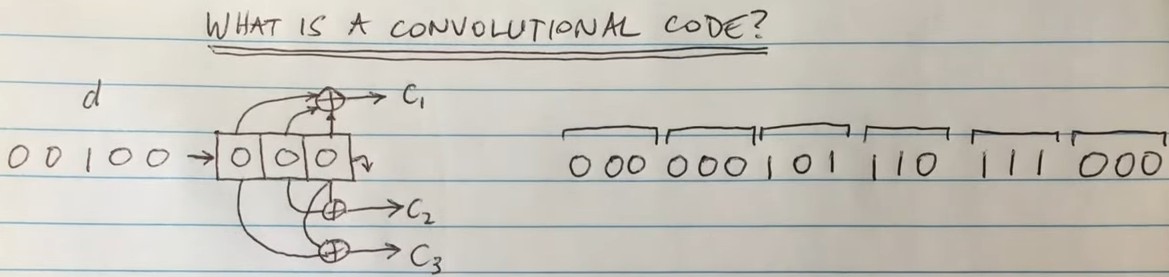
\includegraphics[scale=0.31]{faltungscode}
\end{center}
\subsection{Trellis Diagramm}
Ein Trellis Diagramm ist eine graphische Darstellung eines Faltungscodes. 
Jeder Knoten repräsentiert einen Zustand und jede Kante eine mögliche Transition.
Ein Codewort muss man Rückwärts durch den Baum laufen lassen, um den ursprünglichen Zustand zu finden.

\begin{center}
    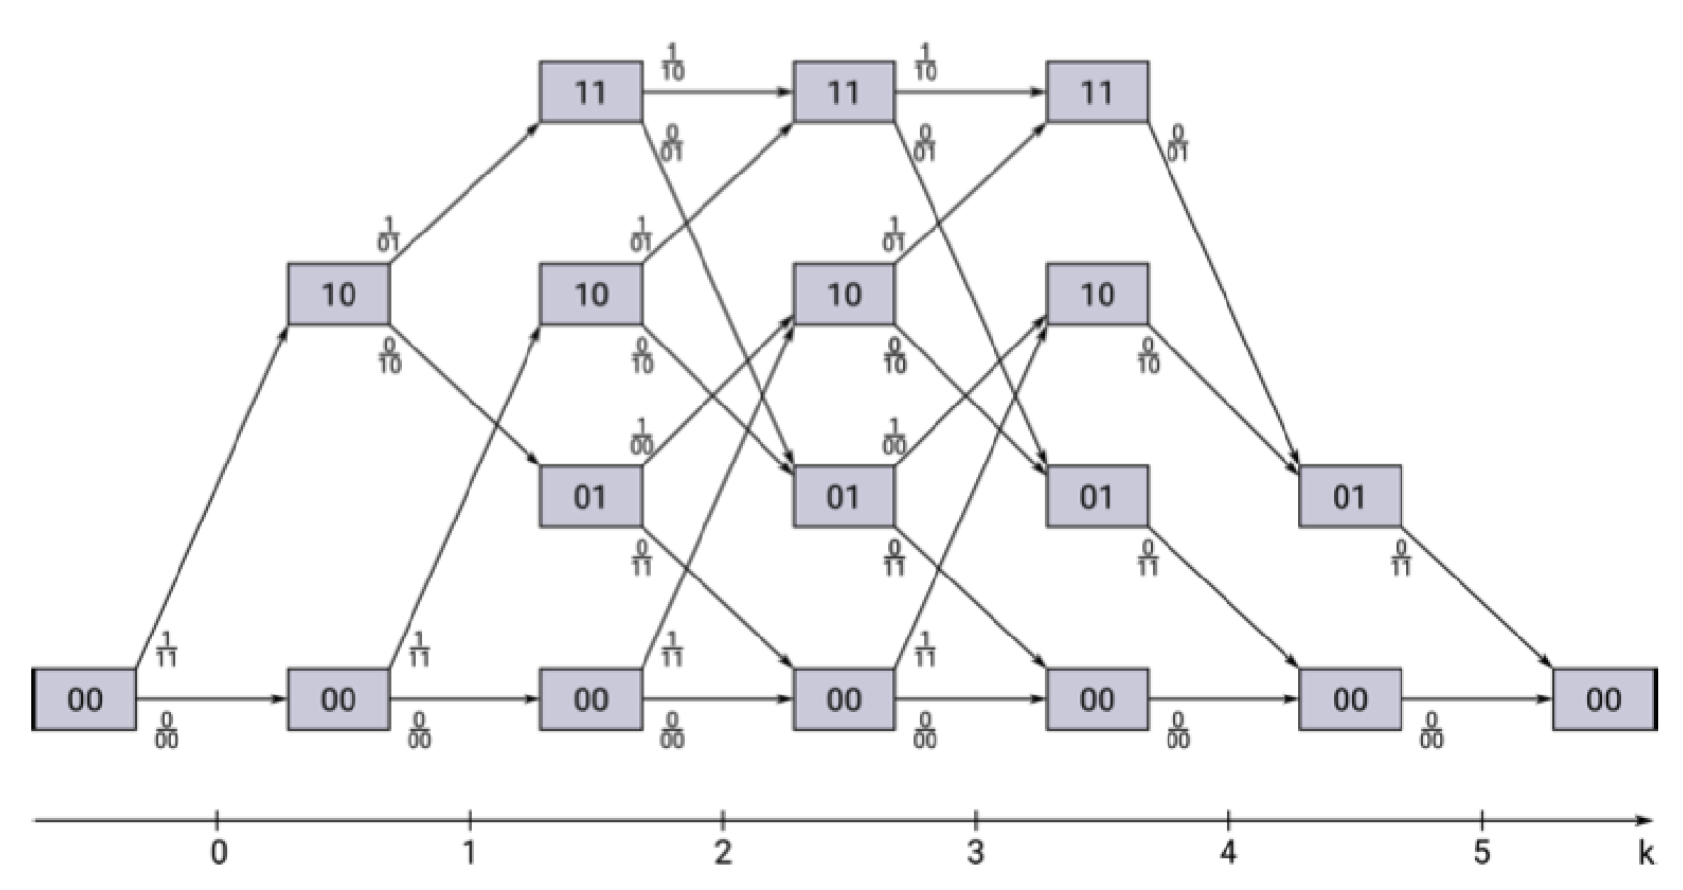
\includegraphics[scale=0.2]{trellis}
\end{center}
\subsection{Optimum Free Distance}
\begin{align*}
    d_{free} = W_{min}
\end{align*}
\\
$W_{min}$ ist das minimale Hamming Gewicht. Berechnung, in dem von
Zustand $[000]$ gestartet wird und der kürzeste Weg zurückgenommen wird.
\begin{center}
    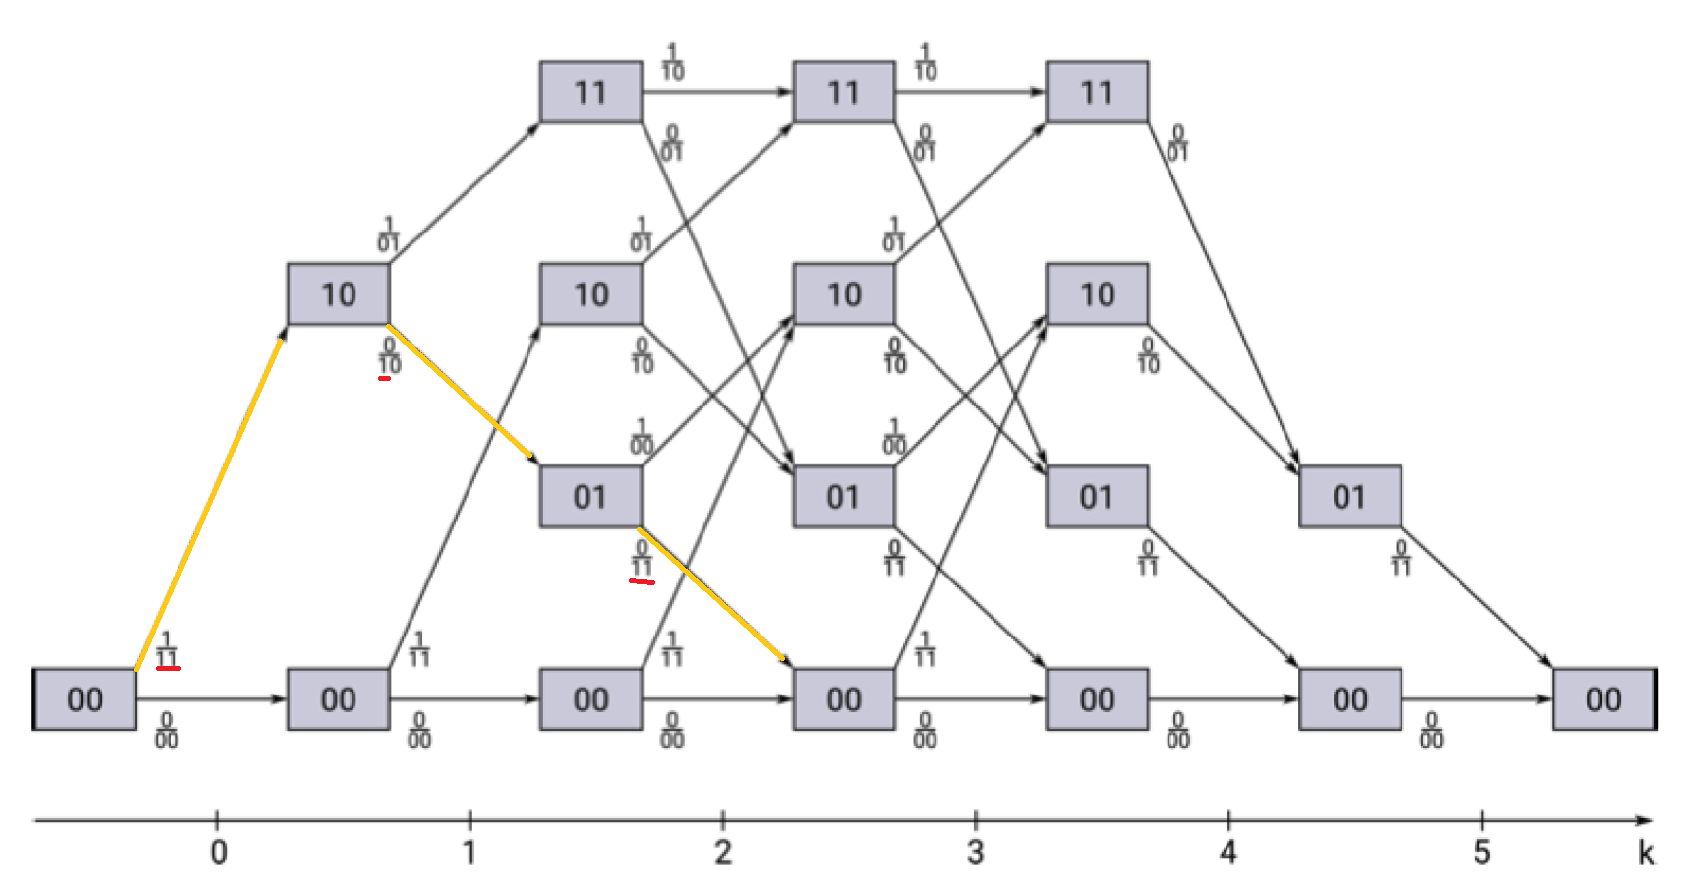
\includegraphics[scale=0.2]{trellis1}
\end{center}
Die Anzahl der Einsen auf dem kürzesten Weg ist $W_{min} = 5$.

\subsection{Coderate $R$}
\begin{align*}
    R = \frac{K}{N} = \frac{K}{2 \cdot (K + m)}
\end{align*}
\subsubsection{Tailbits $m$}
Tailbits sind die $m$ Bits am Ende der Nutzdatenvektoren. Sie sind notwendig, um den Codierer in den 
Anfangszustand zurückzuführen.
\begin{center}
    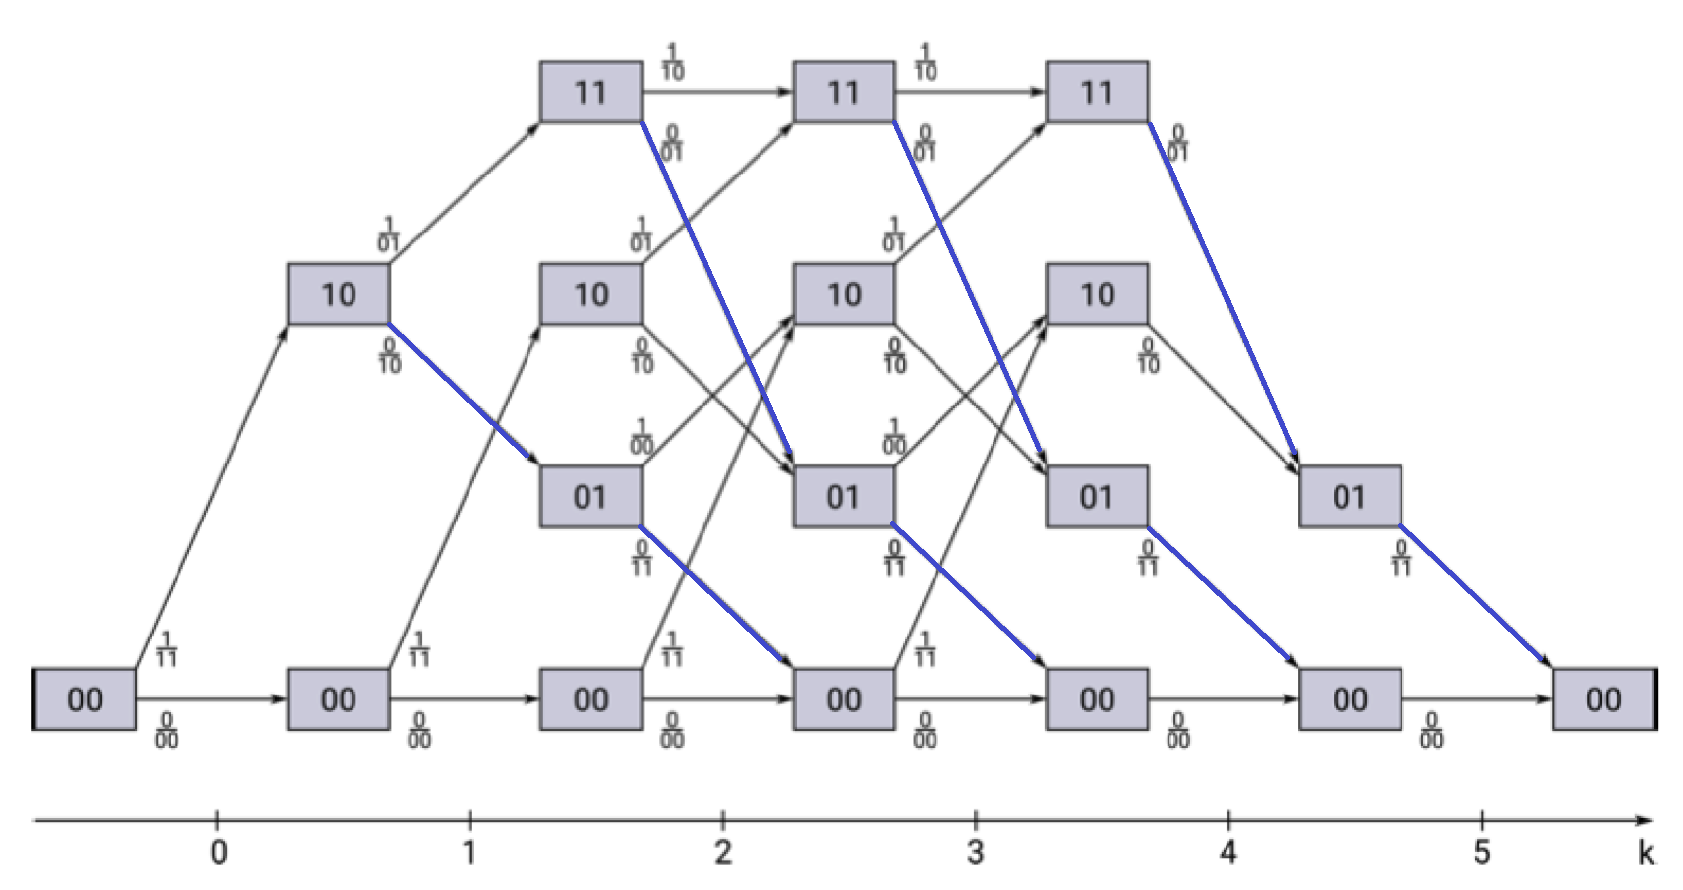
\includegraphics[scale=0.2]{trellis2}
\end{center}
Die Anzahl Tailbits $m$ ist Wie viele Schritte benötigt werden, um von einem 
Zustand in den Anfangszustand zurückzukehren. In diesem Fall sind es $2$ Schritte.
\section{JPEG}
\begin{enumerate}
    \item Y Cr Cb Conversion
    \item 8x8 Pixel Blocks
    \item Discrete Cosine Transformation (DCT)
    \item Quantization
    \item Zig-Zag Scanning
    \item DC and AC Seperation
    \item Run-Length Encoding
    \item Huffman Encoding
    \item JFIF File Creation
\end{enumerate}
\subsection{y $C_r$ $C_b$ Conversion}
Das Bild wird  in Lumineszenz (Y) und Chrominanz ($C_r$, $C_b$) aufgeteilt.
$C_b$ ist der Blauanteil und $C_r$ der Rotanteil.
\subsubsection{Subsampling}
\begin{align*}
    R = \frac{\text{Resultierende Pixel}}{\text{Ursprüngliche Pixel}}
\end{align*}
\begin{itemize}
    \item Subsampling meint, dass in beiden Chrominanz-Ebenen in der
        Horizontalen oder Vertikalen mehrere Pixel zusammengefasst werden.
    \item Der Schema-Indikator gibt die Art des Subsamplings an und hat die
        Form J:a:b (z.B. 4:2:0)
    \item Diese Notation basiert auf einem Referenzbildblock, der J Pixel breit und
        2 Pixel hoch ist. Üblich ist J = 4.
\end{itemize}
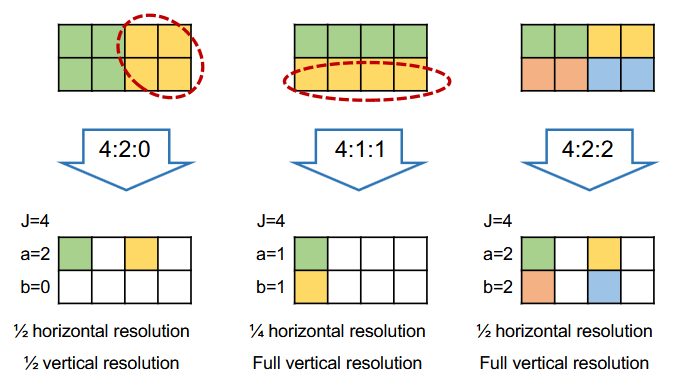
\includegraphics[scale=0.56]{subsampling1}\\
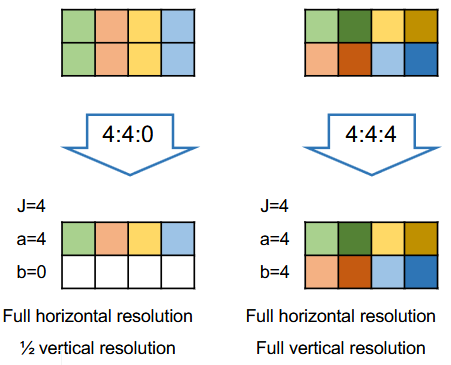
\includegraphics[scale=0.55]{subsampling2}

\subsection{8x8 Pixel Blocks}
Das Bild wird in 8x8 Pixel Blöcke aufgeteilt. Diese Blöcke werden dann einzeln bearbeitet.
\subsection{Discrete Cosine Transformation (DCT)}
Jeder wert der 8x8 Matrix wird durch die DCT in einen Frequenzraum transformiert.
\begin{equation*}
    F(u,v) = \frac{1}{4} \cdot C(u) \cdot C(v) \cdot \sum_{x=0}^{7} \sum_{y=0}^{7} f(x,y) \cdot \cos(\frac{(2x+1)u\pi}{16}) \cdot \cos(\frac{(2y+1)v\pi}{16})
\end{equation*}
Vor DCT:
\begin{center}
    \begin{tabular}{ c c c c c c c c c }
        139 & 144 & 149 & 153 & 155 & 155 & 155 & 155 \\
        144 & 151 & 153 & 156 & 159 & 156 & 156 & 156 \\
        150 & 155 & 160 & 163 & 158 & 156 & 156 & 156 \\
        159 & 161 & 162 & 160 & 160 & 159 & 159 & 159 \\
        159 & 160 & 161 & 162 & 162 & 155 & 155 & 155 \\
        161 & 161 & 161 & 161 & 160 & 157 & 157 & 157 \\
        162 & 162 & 161 & 163 & 162 & 157 & 157 & 157 \\
        162 & 162 & 161 & 161 & 163 & 158 & 158 & 158 \\
    \end{tabular}
\end{center}
Nach DCT ($Q_{vu}$):
\begin{center}
    \begin{tabular}{ c c c c c c c c }
        1260 & -1.0 & -12.1 & -5.2 & 2.1 & -1.7 & -2.7 & 1.3 \\
        -22.6 & -17.5 & -6.2 & -3.2 & -2.9 & -0.1 & 0.4 & -1.2 \\
        -10.9 & -9.3 & -1.6 & 1.5 & 0.2 & -0.9 & -0.6 & -0.1 \\
        -7.1 & -1.9 & 0.2 & 1.5 & 0.9 & -0.1 & -0.0 & 0.3 \\
        -0.6 & -0.8 & 1.5 & 1.6 & -0.1 & -0.7 & 0.6 & 1.3 \\
        1.8 & -0.2 & 1.6 & -0.3 & -0.8 & 1.5 & 1.0 & -1.0 \\
        -1.3 & -0.4 & -0.3 & -1.5 & -0.5 & 1.7 & 1.1 & -0.8 \\
        -2.6 & 1.6 & -3.8 & -1.8 & 1.9 & 1.2 & -0.6 & -0.4 \\
    \end{tabular}
\end{center}
\subsection{Quantization}
Die Frequenzanteile von der DCT werden nun durch eine Quantizationstabelle ($Q_{vu}$) geteilt. Die Quantizationstabelle
wird je nach JPEG Verfahren anders gewählt. Quantizationstabelle für Luminanz:
\begin{center}
    \begin{tabular}{ c c c c c c c c }
        16 & 11 & 10 & 16 & 24 & 40 & 51 & 61 \\
        12 & 12 & 14 & 19 & 26 & 58 & 60 & 55 \\
        14 & 13 & 16 & 24 & 40 & 57 & 69 & 56 \\
        14 & 17 & 22 & 29 & 51 & 87 & 80 & 62 \\
        18 & 22 & 37 & 56 & 68 & 109 & 103 & 77 \\
        24 & 35 & 55 & 64 & 81 & 104 & 113 & 92 \\
        49 & 64 & 78 & 87 & 103 & 121 & 120 & 101 \\
        72 & 92 & 95 & 98 & 
    \end{tabular}
\end{center}
Nun nimmt man die 8x8 Tabelle von nach der DCT und teilt sie durch die Quantizationstabelle bzw.
Folgende Funktion:
\begin{align*}
    F_{vu} = round(F_{vu}/Q_{vu})
\end{align*}

\begin{center}
    \begin{tabular}{ c c c c c c c c }
        79 & 0 & -1 & 0 & 0 & 0 & 0 & 0 \\
        -2 & -1 & 0 & 0 & 0 & 0 & 0 & 0 \\
        -1 & -1 & 0 & 0 & 0 & 0 & 0 & 0 \\
        -1 & 0 & 0 & 0 & 0 & 0 & 0 & 0 \\
        0 & 0 & 0 & 0 & 0 & 0 & 0 & 0 \\
        0 & 0 & 0 & 0 & 0 & 0 & 0 & 0 \\
        0 & 0 & 0 & 0 & 0 & 0 & 0 & 0 \\
        0 & 0 & 0 & 0 & 0 & 0 & 0 & 0
    \end{tabular}
\end{center}



\section{Audiocodierung}



\end{multicols*}
\end{document}